% Written by code/scripts/lc5m_section.py (scripts/lc5m_section.sh); edits here are overwritten.
\clearpage
\paragraph{LC5m: LC5 with a Muon floor (in progress).} LC5m is LC5 (\cref{tab:lc}) with a hard constraint: every singular value of its update lies between Muon's value and the exact $s^{-0.3}$.

\begin{table}[H]
\centering
\small
\caption{LC5m, one row per data order. GPU minutes until the validation loss first reaches 1.3391, as in \cref{tab:negp,tab:lc}; ms per step: Muon 117, LC5 123, exact 1081, AdamW 107, LC5m 123 (timed as LC5 until its own timing pilot has run). Exact: exact SVD, $p=-0.3$. running: not finished; --: not run. Mean: over the orders where LC5m has finished (none yet).}
\label{tab:lc5m}
\setlength{\tabcolsep}{3.5pt}
\begin{tabular}{l ccccc ccccc}
\toprule
 & \multicolumn{5}{c}{final val.\ loss} & \multicolumn{5}{c}{GPU min.\ to 1.3391} \\
\cmidrule(lr){2-6}\cmidrule(lr){7-11}
order & LC5m & Muon & LC5 & exact & AdamW & LC5m & Muon & LC5 & exact & AdamW \\
\midrule
d0 & running & 1.3049 & 1.3108 & 1.3002 & 1.3391 & running & 14.6 & 16.0 & 131.8 & 17.9 \\
d1 & running & 1.3070 & 1.3092 & 1.3055 & 1.3462 & running & 14.7 & 15.7 & 133.9 & never \\
d2 & running & 1.3138 & 1.3126 & 1.3023 & 1.3446 & running & 15.1 & 15.9 & 132.6 & never \\
d3 & running & 1.3084 & -- & -- & 1.3496 & running & 14.9 & -- & -- & never \\
d4 & running & 1.3090 & -- & -- & 1.3403 & running & 15.1 & -- & -- & never \\
\midrule
mean & -- & -- & -- & -- & -- & -- & -- & -- & -- & -- \\
\bottomrule
\end{tabular}
\end{table}

\begin{figure}[H]
\centering
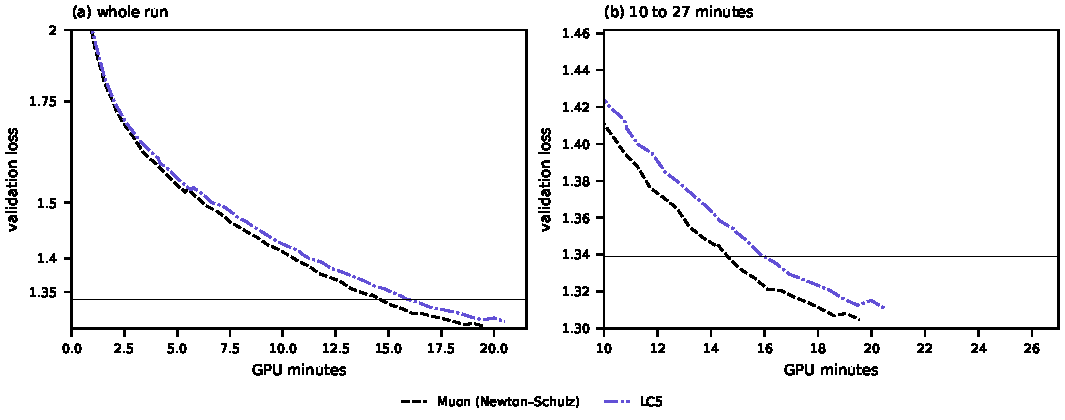
\includegraphics[width=\linewidth]{ts10m/lc5m_gpu_time_ce.pdf}
\caption{As \cref{fig:gputime}, for LC5m, LC5 and Muon on data order 0 (no LC5m run has finished yet).}
\label{fig:lc5m}
\end{figure}
